\documentclass[a4paper,14pt]{extarticle}

\usepackage[utf8x]{inputenc}
\usepackage[T1]{fontenc}
\usepackage[russian]{babel}
\usepackage{hyperref}
\usepackage{indentfirst}
\usepackage{here}
\usepackage{array}
\usepackage{graphicx}
\usepackage{caption}
\usepackage{subcaption}
\usepackage{chngcntr}
\usepackage{amsmath}
\usepackage{amssymb}
\usepackage[left=2cm,right=2cm,top=2cm,bottom=2cm,bindingoffset=0cm]{geometry}
\usepackage{multicol}
\usepackage{multirow}
\usepackage{titlesec}
\usepackage{listings}
\usepackage{color}
\usepackage{enumitem}
\usepackage{cmap}
\usepackage{underscore}

\definecolor{green}{rgb}{0,0.6,0}
\definecolor{gray}{rgb}{0.5,0.5,0.5}
\definecolor{purple}{rgb}{0.58,0,0.82}

\lstdefinelanguage{none}{}

\lstset{
	language={SQL},
	inputpath={../sql/},
	backgroundcolor=\color{white},
	commentstyle=\color{green},
	keywordstyle=\color{blue},
	numberstyle=\scriptsize\color{gray},
	stringstyle=\color{purple},
	basicstyle=\small,
	breakatwhitespace=false,
	breaklines=true,
	captionpos=b,
	keepspaces=true,
	numbers=left,
	numbersep=5pt,
	showspaces=false,
	showstringspaces=false,
	showtabs=false,
	tabsize=4,
	texcl=true,
	frame=single
}

\renewcommand{\le}{\ensuremath{\leqslant}}
\renewcommand{\leq}{\ensuremath{\leqslant}}
\renewcommand{\ge}{\ensuremath{\geqslant}}
\renewcommand{\geq}{\ensuremath{\geqslant}}
\renewcommand{\epsilon}{\ensuremath{\varepsilon}}
\renewcommand{\phi}{\ensuremath{\varphi}}
\renewcommand{\thefigure}{\arabic{figure}}
\newcommand{\code}[1]{\texttt{#1}}
\newcommand{\caret}{\^{}}

\titleformat*{\section}{\large\bfseries} 
\titleformat*{\subsection}{\normalsize\bfseries} 
\titleformat*{\subsubsection}{\normalsize\bfseries} 
\titleformat*{\paragraph}{\normalsize\bfseries} 
\titleformat*{\subparagraph}{\normalsize\bfseries} 

\counterwithin{figure}{section}
\counterwithin{equation}{section}
\counterwithin{table}{section}
\newcommand{\sign}[1][5cm]{\makebox[#1]{\hrulefill}}
\newcommand{\equipollence}{\quad\Leftrightarrow\quad}
\newcommand{\no}[1]{\overline{#1}}
\graphicspath{{/pics/}}
\captionsetup{justification=centering,margin=1cm}
\def\arraystretch{1.3}
\setlength\parindent{5ex}
\titlelabel{\thetitle.\quad}

\setitemize{topsep=0.5em, itemsep=0em}
\setenumerate{topsep=0.5em, itemsep=0em}

\begin{document}

\begin{titlepage}
\begin{center}
	Санкт-Петербургский Политехнический Университет Петра Великого\\[0.3cm]
	Институт компьютерных наук и технологий \\[0.3cm]
	Кафедра компьютерных систем и программных технологий\\[4cm]
	
	\textbf{ОТЧЕТ}\\ 
	\textbf{по лабораторной работе}\\[0.5cm]
	\textbf{<<Разработка структуры базы данных>>}\\[0.1cm]
	Базы данных\\[3.0cm]
\end{center}

\begin{flushright}
	\begin{minipage}{0.45\textwidth}
		\textbf{Работу выполнил студент}\\[3mm]
		группа 43501/3 \hfill Крылов И.С.\\[5mm]
		\textbf{Работу принял преподаватель}\\[5mm]
		\sign[3cm] \hfill Мяснов А.В. \\[5mm]
	\end{minipage}
\end{flushright}

\vfill

\begin{center}
	Санкт-Петербург\\[0.3cm]
	\the\year
\end{center}
\end{titlepage}

\addtocounter{page}{1}

\tableofcontents
\newpage

\section{Цель работы}

Познакомиться с основами проектирования схемы БД, способами организации данных в SQL-БД.

\section{Программа работы}

\begin{enumerate}
	\item Создание проекта для работы в GitLab.
	\item Выбор задания (предметной области), описание набора данных и требований к хранимым данным в свободном формате в Wiki своего проекта в GitLab.
	\item Формирование в свободном формате (предпочтительно в виде графической схемы) схемы БД, соответствующей заданию. Должно получиться не менее 7 таблиц.
	\item Согласование с преподавателем схемы БД. Обоснование принятых решений и соответствия требованиям выбранного задания. 
	\item Выкладывание схемы БД в свой проект в GitLab.
	\item Демонстрация результатов преподавателю.
\end{enumerate}

\section{Выполнение работы}


\subsection{Выбор предметной области}

Для выполнения работы была выбрана тема задания онлайн магазина видеоигр. База данных хранит общие сведения об игре, предоставляющие краткое описание самой игры, вместе с системными требованиями к оборудованию на котором возможен запуск игры.

\subsection{Описание таблиц}

В процессе проектирования схемы базы данных были выделены следующие сущности:
\begin{itemize}
	\item \code{game} -- хранит общую информацию об игреЮ такую как: \code{price} - стоимость игры, системные требования \code{system_requirements}, \code{developer} - разработчика игры, \code{release_date} - дата выпуска.
	
	\item \code{system_requirements} -- хранит информацию о минимальных \code{minimal_requirements} и оптимальных \code{optimal_requirements} системных требованиях.
\end{itemize}
	

\subsection{Структура базы данных}

\begin{figure}[H]
	\centering
	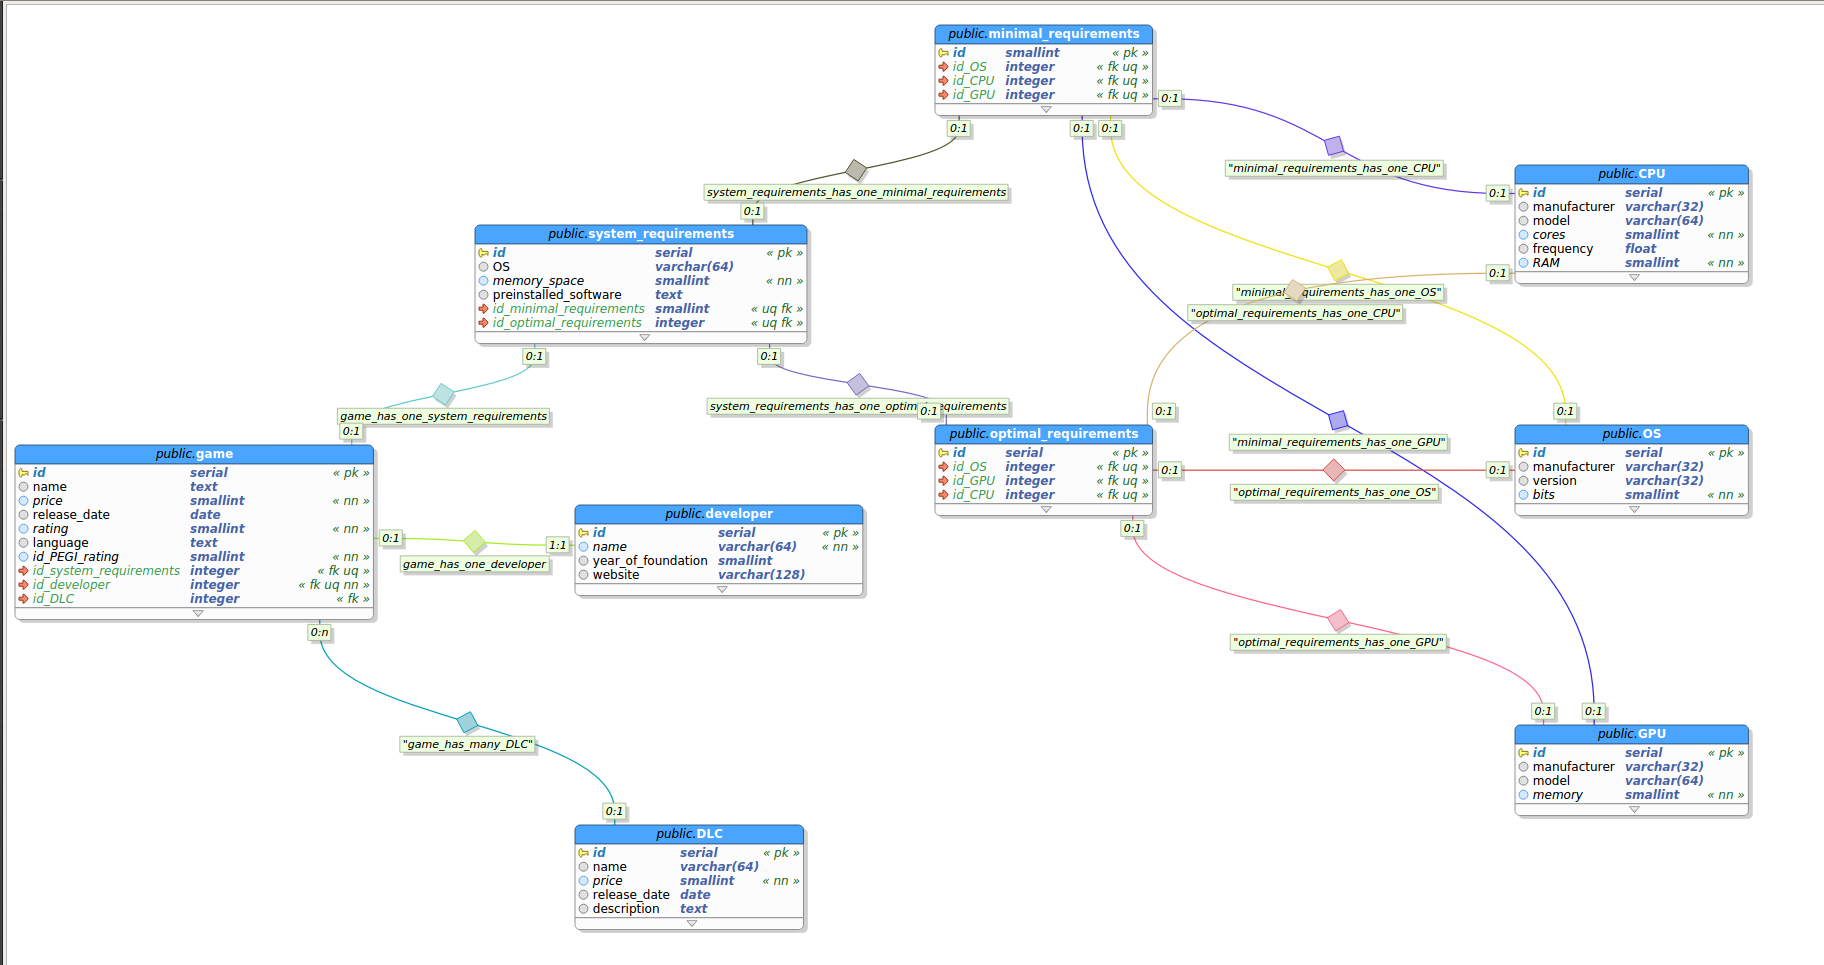
\includegraphics[width=\linewidth]{../pics/scheme.png}
\end{figure}

\section{Выводы}

В ходе выполнения данной работы была спроектирована и согласована с преподавателем база данных для онлайн магазина видеоигр. Было выделено несколько основные сущностей, таких как игра, разработчик и системные требования, а также множество вспомогательных таблиц для хранения информации о дополнительном игровом контенте и подробных системных требований.

\end{document}